\chapter{Introduction to carbon materials}
	As graphene is composed of \textit{sp\textsubscript{2}-hybridized} carbon atoms we need want to introduce some fundamentals of the carbon properties.
	\section{Carbon Atom}
		Carbon is the $6^{th}$ element in the $14^{th}$ group of the periodic table (\ref{fig:periodicTable}). Therefore it is nonmetallic, tetravalent and constituted of 6 protons and electrons. There are three natural occurring isotopes, with $^{12}_{\phantom{0}6}C$, $^{13}_{\phantom{0}6}C$ being stable and $^{14}_{\phantom{0}6}C$ being radiative with an half life of 5.730 years. $^{14}_{\phantom{0}6}C$ $\beta$ decays to nitrogen and is used for historical dating. 
		The most common allotropes of Carbon are graphite, graphene and diamond. Diamond and graphene have the highest thermal conductivity of all known materials. The electron configuration in the ground state of carbon is $1s^22s^22p^2$, i.e. there are two electrons in the 1s orbital, which are irrelevant for chemical bondings, in addition to four electrons in the outer shell. The 2p orbital is roughly 4eV higher than the 2s orbital, therefore it is energetic favorable to put two electrons in the 2s and two electrons the 2p orbitals. However, carbon tends to fill one 2p orbital with an electron from the 2s orbital, in the presence of other atoms like H, O or C, which leads to 4 equal quantum states $|2s \rangle$, $|2p_x \rangle$, $|2p_y \rangle$ and $|2p_z \rangle$. A quantum-mechanical superposition of the state $|2s \rangle$ with $n |2p_i \rangle$ states is called sp\textsuperscript{n} hybridization.
		\begin{figure}[htbp]
			\begin{minipage}[b]{0.4\textwidth} 
				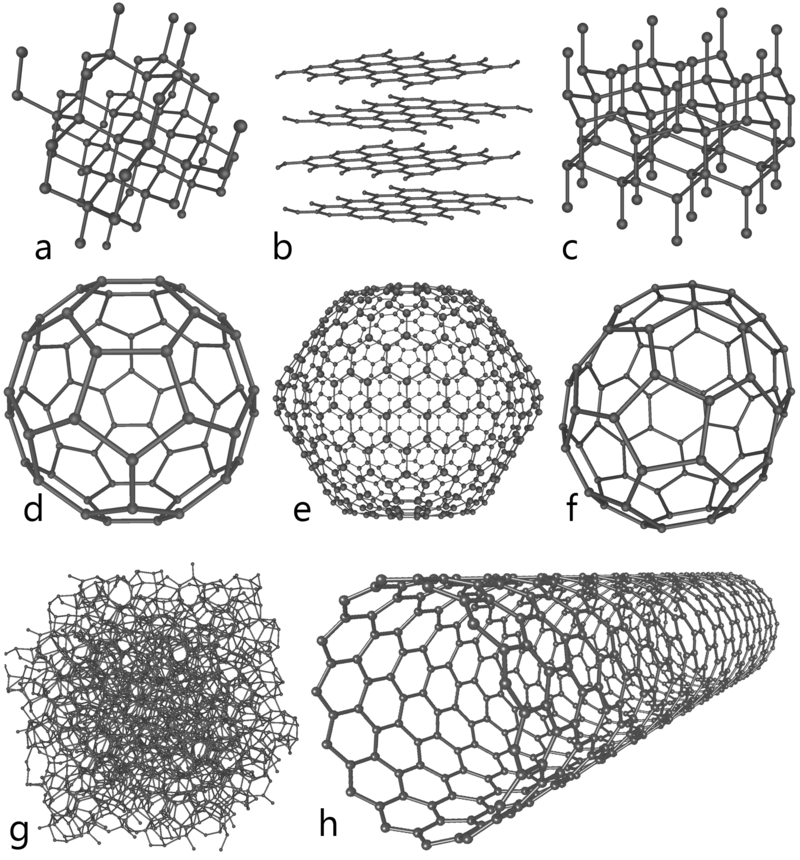
\includegraphics[width=\textwidth]{figures/Carbon/carbonAllotropes.png}		
			\end{minipage}
			% Auffüllen des Zwischenraums
			\hfill
			% minipage mit Grafik
			\begin{minipage}[t]{0.5\textwidth}
			\centering
			% \textwidth bezieht sich nun auf die Minipage
			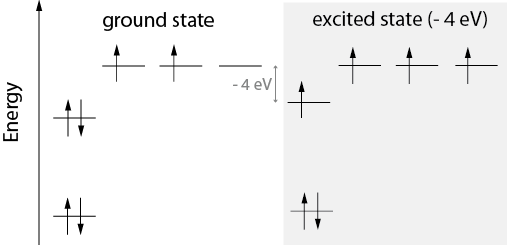
\includegraphics[width=\textwidth]{figures/Carbon/carbonElectronicConfiguration.png}
			\end{minipage}
			\caption{\textbf{Left :} Allotropes of Carbon : a) diamond, b) graphite, c) Ionsdaleite, d-f) fullerences, g) amorphous carob, h) carbon, nanotube. Figure taken from \cite{enWikiAllotropesOfCarbon}. \\
			\textbf{Right :} Comparison between the electronic configuration of carbon in the ground state and in the excited state.}		
		\end{figure}

		\subsection{sp\textsuperscript{1}-hybridization}
			\begin{figure}[h]
				\centering
				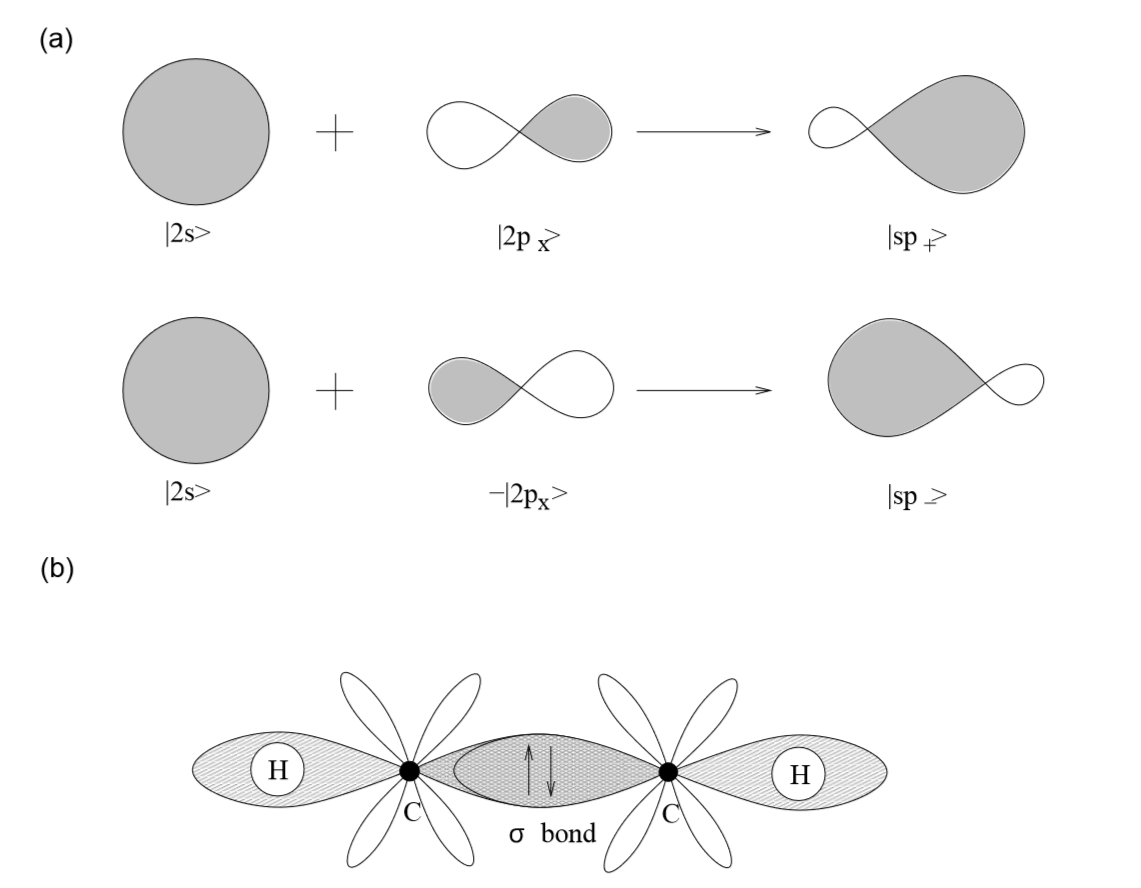
\includegraphics[width=0.9\textwidth]{figures/Carbon/carbonHybridization.png}
				\caption{\textbf{a :} First hybridization of the carbon atom \\
				\textbf{b :} Ethyne molecule with one sigma and two $\pi$ bonds (not shown).\\
				Figure taken from \cite{grapheneIntroduction}.}
				\label{fig:carbonHybridization}
			\end{figure}	
			In the sp\textsuperscript{1} hybridization a $|2s \rangle$ orbital mixes with one of the three $|2p \rangle$ states. For example:
			\begin{align}
				| sp_+ \rangle &= \tfrac{1}{\sqrt{2}} (|2s \rangle + |2p_x \rangle) \\
				| sp_- \rangle &= \tfrac{1}{\sqrt{2}} (|2s \rangle - | 2p_x \rangle)
			\end{align}
			The two orbitals mix into two new one with the geometrical appearance displayed in Figure \ref{fig:carbonHybridization}. The $|sp_+ \rangle$ and $|sp_- \rangle$ orbitals can now be used to form strong $\sigma$ bounds as in acetylene (ethyne) ($HC \equiv CH$). The rest of the three p orbitals can now compose $\pi$-bounds.
			
			
					
		\subsection{sp\textsuperscript{2}-hybridization}
			\label{sec:sp2hybridisation}
			\begin{figure}[h]
				\centering
				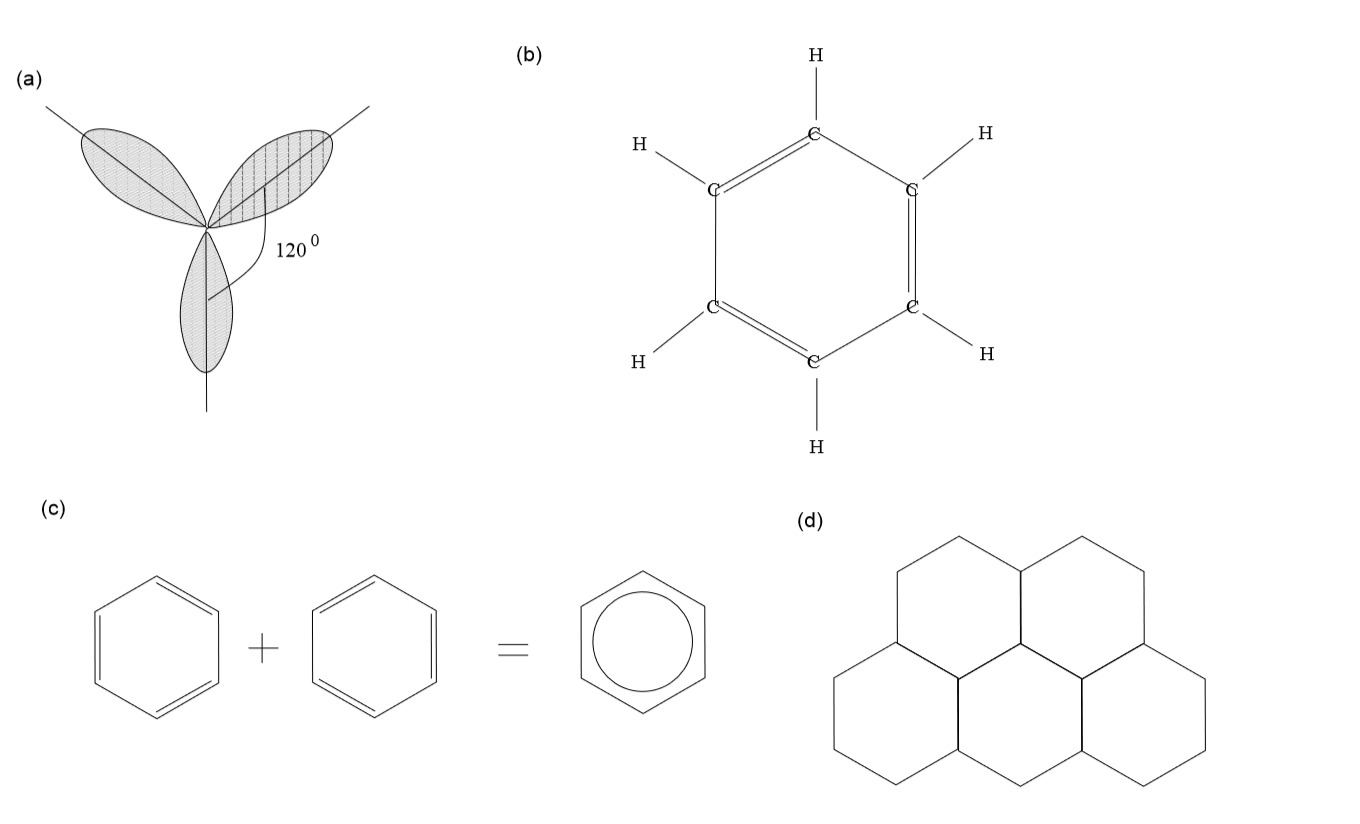
\includegraphics[width=0.9\textwidth]{figures/Carbon/carbonHybridization2.png}
				\caption{\textbf{a :} Schematic view of the sp\textsuperscript{2} hybridization \\
				\textbf{b :} Benzene ring \\
				\textbf{c :} the $\pi$ bonds of the benzene ring arise out of a superposition of two configurations and therefore to delocalised electrons \\
				\textbf{d :} graphene can be viewed the tiling of benzene rings, where the H atoms are replaced by neighbored carbon atoms.\\
				Figure taken from \cite{grapheneIntroduction}.}
				\label{fig:carbonHybridization2}
			\end{figure}	
			The graphene lattice consists of sp\textsuperscript{2} hybridized carbon atoms. Sp\textsuperscript{2} hybridization means the merging of a $| 2s \rangle$ state with two $| p \rangle$ orbitals. For example the mixing of the $| 2s  \rangle$ orbital with the $| p_x \rangle$ and the $|p_y \rangle$ states.
			\begin{align}
				| sp_1^2 \rangle &= \tfrac{1}{\sqrt{3}} | 2s \rangle - \sqrt{\tfrac{2}{3}} | 2p_y \rangle, \\
				| sp_2^2 \rangle &= \tfrac{1}{\sqrt{3}} | 2s \rangle + \sqrt{\tfrac{2}{3}} (\tfrac{\sqrt{3}}{2} |2 p_x \rangle + \tfrac{1}{2} | 2p_y \rangle), \\
				|sp_3^2 \rangle &= - \tfrac{1}{\sqrt{3}} | 2s \rangle + \sqrt{\tfrac{2}{3}} ( - \tfrac{\sqrt{3}}{2} | 2p_x \rangle + \tfrac{1}{2} | 2 p_y \rangle)
			\end{align}
			The three sp\textsuperscript{2} orbitals are located in the xy plane having mutual 120 degree angles. The remaining not hybridized ($p_z$) orbital is perpendicular to the plane. An example for the sp\textsuperscript{2} hybridization is the benzene ring. It is an hexagon with six sp\textsuperscript{2} hybridized carbon atoms at its corners, lined by $\sigma$ bonds, while having three $\pi$ bonds. Graphene can be seen as tilings of benzene where the hydrogens are substituted by carbon atoms from the neighboring carbon hexagons.		

	
	\section{Crystal Structure of graphite and graphene}
		We will now regard the \textit{honeycomb lattice} of graphene and if we consider a three dimensional graphene stacking the structure of \textit{graphite}.
		
		\subsection{Honeycomb lattice}
			As discussed in \ref{sec:sp2hybridisation} graphene condenses in a planar honeycomb lattice due to its sp\textsuperscript{2} hybridization. Consequently every carbon has three $\sigma$ bonds and one $\pi$ bond, which also creates a delocalised $\pi$ system being responsible for the extraordinary good conductivity of graphene. Graphene naturally consists of two hexagonal (trigonal) sub-lattices A and B. For creating a \textit{Bravais lattice} one has to use a two-atom basis with a distance of 0.142nm, representing the average of the single (C-C) and double (C=C) bondings of benzene, which itself can be seen as hydrogen substituted graphene fragments.		
			\begin{figure}[ht]
				\centering
				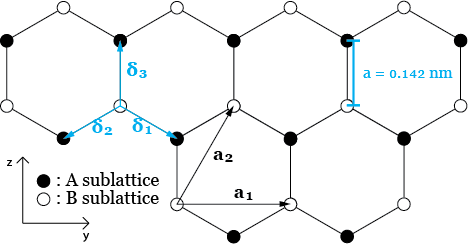
\includegraphics[width=0.6\textwidth]{figures/Carbon/grapheneLattice.png}
				\caption{Honeycomb lattice. The vectors $\vec{v_1}$, $\vec{v_2}$ and $\vec{v_3}$ connect the basis atoms seperated by a distance a. The vectors $\vec{a_1}$ and $\vec{a_2}$ are basis vectors of the triangular Bravais lattice.}
				\label{fig:grapheneHoneycomb}
			\end{figure}			
			The three vectors, which transfer sub-lattice A into B are given by:
			\begin{align}
				\label{eq:grapheneDisplacement}
				\boldsymbol{\delta_1} = \frac{a}{2} (\sqrt{3} \vec{e_y} - \vec{e_z}) && \boldsymbol{\delta_2} = - \frac{a}{2} (\sqrt{3} \vec{e_y} + \vec{e_z}) && \boldsymbol{\delta_3} = a \vec{e_z}.
			\end{align}
			Whereas the Bravais lattice vectors are :
			\begin{align}
				\vec{a_1} = \sqrt{3} a \vec{e_y} && \vec{a_2} =  \frac{\sqrt{3}a}{2} (\vec{e_y} + \sqrt{3} \vec{e_z}).
			\end{align}
			From the lattice shown in \ref{fig:grapheneHoneycomb} one can obtain some more important properties like the lattice spacing $\tilde{a} = \sqrt{3}a = 0.24$nm, the surface of the primitive Cell (\ref{sec:primitiveCell}) $A_{pc} = \frac{\sqrt{3}\tilde{a}^2}{2} = 0.051$nm$^2$, the density of carbon atoms $n_c = \frac{2}{A_{pc}} = 39$nm$^{-2}$ and the electron density $n_\pi = n_c = 39$nm$^{-2} = 3.9\cdot 10^{15}$cm$^{-2}$. One have to mention that the electron density in graphene, calculated from the Bravais lattice, \textbf{is not} equal to the carrier density we are going to calculate in the following chapters. 
			\begin{figure}[ht]
				
				\centering
				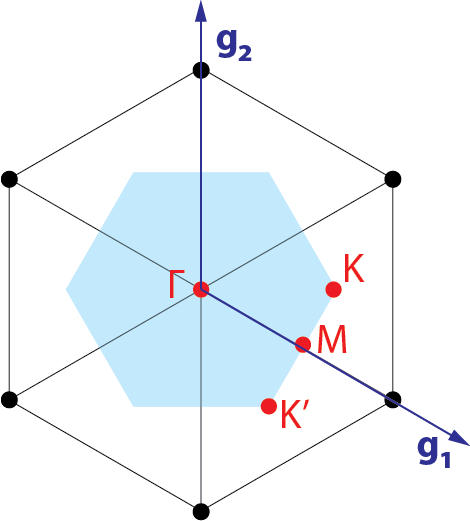
\includegraphics[width=0.5\textwidth]{figures/Carbon/grapheneBrillouin.png}
				\caption{Reciprocal lattice of the triangular Bravais lattice. The blue shaded surface denotes the first brillouin zone. Moreover one can see the lattice vectors $\vec{g_1}$ and $\vec{g_2}$ and the crystallographic points $\Gamma$, K, M and K'.}
				\label{fig:grapheneBrillouin}
			\end{figure}
			The reciprocal lattice (\ref{sec:reciprocalLattice}) is spanned by the vectors 
			\begin{align}
				\vec{g_1} = \frac{2\pi}{\sqrt{3}a} (\vec{e_y} - \frac{\vec{e_z}}{\sqrt{3}}) && \vec{g_2} = \frac{4 \pi}{3a} \vec{e_z}.
			\end{align}
			The correctness of the reciprocal vectors can be easily shown by 
			\begin{align}
				\vec{a_i} \cdot \vec{g_i} = 2 \pi \delta_{ij} && i,j \in {1,2}
			\end{align}
			In Fig. \ref{fig:grapheneBrillouin} one can see the reciprocal lattice vectors, the Brillouin zone, which is blue shaded, and the supersymmetry points $\Gamma$, K, M and K'.
			\begin{equation}
				\vec{K} = \frac{4 \pi}{3 \sqrt{3}a}\vec{e_y}
			\end{equation}
			These crystallographic points play an essential role for the electronic properties, as will be discussed in the following chapters. Having talked about the basic features we will now continue with the structure of graphite, which layers graphene lattices. Further information about graphene can be taken from \cite{grapheneProperties}.
		
		\subsection{Graphene stacking}
			Graphite consists of stacked graphene layers. We distinguish ordered graphite from turbostatic graphite (graphite which has parallel graphene layers with a chaotic order). We will only do calculations for the ordered graphene layers, which contains reflexion symmetry (z = -z). In this case the distance between two neighboring layers is $d = 2.4a = 0.34nm$. Two neighboring layers are always shifted so that some carbon atoms of one layer are placed above the center of the hexagons of the other one. Their displacement is given by $\delta_i$ or $-\delta_i$, used in equation \ref{eq:grapheneDisplacement}.
			
		\begin{figure}[ht]
			\label{fig:grapheneStacking}
			\centering
			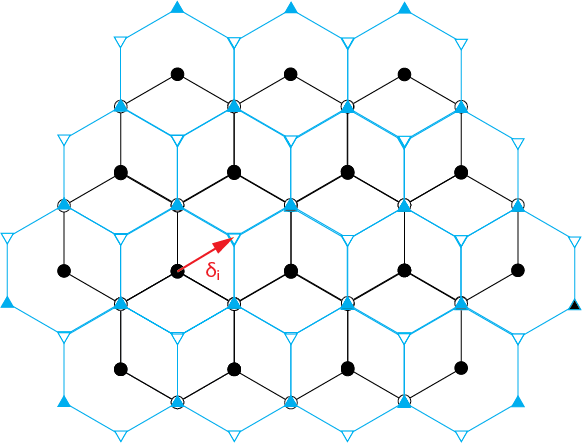
\includegraphics[width=0.5\textwidth]{figures/Carbon/grapheneStacking.png}
			\caption{Two graphene layers shifted by $\delta_i$}
		\end{figure}
		
		\begin{figure}[ht]
			\label{fig:graphiteDisordered}
			\centering
			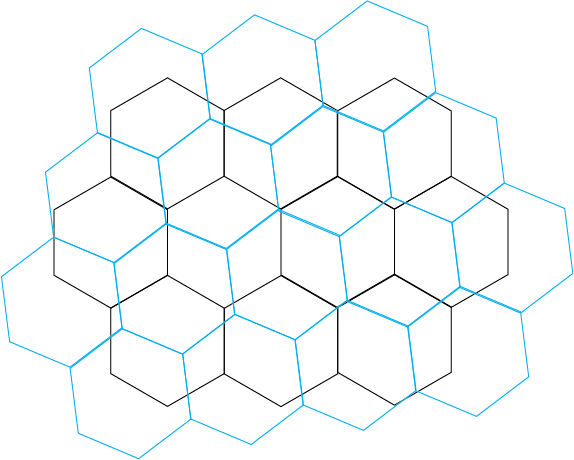
\includegraphics[width=0.9\textwidth]{figures/Carbon/graphiteDisordered.png}
			\caption{Two layers of disordered graphite.}
		\end{figure}
		

		
			
	
	